\documentclass[a4paper]{report}\usepackage[]{graphicx}\usepackage[]{color}
%% maxwidth is the original width if it is less than linewidth
%% otherwise use linewidth (to make sure the graphics do not exceed the margin)
\makeatletter
\def\maxwidth{ %
  \ifdim\Gin@nat@width>\linewidth
    \linewidth
  \else
    \Gin@nat@width
  \fi
}
\makeatother

\definecolor{fgcolor}{rgb}{0.345, 0.345, 0.345}
\newcommand{\hlnum}[1]{\textcolor[rgb]{0.686,0.059,0.569}{#1}}%
\newcommand{\hlstr}[1]{\textcolor[rgb]{0.192,0.494,0.8}{#1}}%
\newcommand{\hlcom}[1]{\textcolor[rgb]{0.678,0.584,0.686}{\textit{#1}}}%
\newcommand{\hlopt}[1]{\textcolor[rgb]{0,0,0}{#1}}%
\newcommand{\hlstd}[1]{\textcolor[rgb]{0.345,0.345,0.345}{#1}}%
\newcommand{\hlkwa}[1]{\textcolor[rgb]{0.161,0.373,0.58}{\textbf{#1}}}%
\newcommand{\hlkwb}[1]{\textcolor[rgb]{0.69,0.353,0.396}{#1}}%
\newcommand{\hlkwc}[1]{\textcolor[rgb]{0.333,0.667,0.333}{#1}}%
\newcommand{\hlkwd}[1]{\textcolor[rgb]{0.737,0.353,0.396}{\textbf{#1}}}%

\usepackage{framed}
\makeatletter
\newenvironment{kframe}{%
 \def\at@end@of@kframe{}%
 \ifinner\ifhmode%
  \def\at@end@of@kframe{\end{minipage}}%
  \begin{minipage}{\columnwidth}%
 \fi\fi%
 \def\FrameCommand##1{\hskip\@totalleftmargin \hskip-\fboxsep
 \colorbox{shadecolor}{##1}\hskip-\fboxsep
     % There is no \\@totalrightmargin, so:
     \hskip-\linewidth \hskip-\@totalleftmargin \hskip\columnwidth}%
 \MakeFramed {\advance\hsize-\width
   \@totalleftmargin\z@ \linewidth\hsize
   \@setminipage}}%
 {\par\unskip\endMakeFramed%
 \at@end@of@kframe}
\makeatother

\definecolor{shadecolor}{rgb}{.97, .97, .97}
\definecolor{messagecolor}{rgb}{0, 0, 0}
\definecolor{warningcolor}{rgb}{1, 0, 1}
\definecolor{errorcolor}{rgb}{1, 0, 0}
\newenvironment{knitrout}{}{} % an empty environment to be redefined in TeX

\usepackage{alltt}
\usepackage[utf8]{inputenc}
\usepackage[T1]{fontenc}
\usepackage{RJournal_edited}
\usepackage{amsmath,amssymb,array}
\usepackage{booktabs}
%\VignetteIndexEntry{Introduction to rotations}
%\VignetteDepends{knitr}
%\VignetteEngine{knitr::knitr}

%% load any required packages here
\usepackage{bm,subcaption,amsfonts}
\IfFileExists{upquote.sty}{\usepackage{upquote}}{}
\begin{document}


%% do not edit, for illustration only
\sectionhead{}
\volume{}
\volnumber{}
\year{}
\month{}
\begin{article}
%% replace RJtemplate with your article
\title{\pkg{apsimr}: Edit, run and evaluate APSIM simulatsion from R easily}
\author{by Bryan Stanfill}

\maketitle
\end{article}

\section{Introduction}

\section{Run}

To run an APSIM simulation the only required argument is the path to the APSIM executible with \code{exe}.  Two additional arguments are optional.  \code{wd} specifies the working directory to which the results \verb=.out= file will be written to which is set to the current working direcory by default.  \code{files} is the list of \verb=.apsim= simulation files to be run which is set to all files in the specified working directory by default.
\begin{knitrout}
\definecolor{shadecolor}{rgb}{0.969, 0.969, 0.969}\color{fgcolor}\begin{kframe}
\begin{alltt}
\hlstd{exe} \hlkwb{<-}\hlstr{"C:/Program Files (x86)/Apsim76-r3376/Model/Apsim.exe"}
\hlstd{wd} \hlkwb{<-} \hlstr{"~/APSIM"}
\hlstd{to_run} \hlkwb{<-} \hlkwd{c}\hlstd{(}\hlstr{"Centro.apsim"}\hlstd{,} \hlstr{"Continuous Wheat.apsim"}\hlstd{)}
\hlstd{results} \hlkwb{<-} \hlkwd{apsim}\hlstd{(}\hlkwc{exe} \hlstd{= exe,} \hlkwc{wd} \hlstd{= wd,} \hlkwc{files} \hlstd{= to_run)}
\end{alltt}
\end{kframe}
\end{knitrout}


\section{Edit}

The file I want to edit is called "Canopy.apsim" which is in the directory "$\sim$/APSIM"
\begin{knitrout}
\definecolor{shadecolor}{rgb}{0.969, 0.969, 0.969}\color{fgcolor}\begin{kframe}
\begin{alltt}
\hlstd{file} \hlkwb{<-} \hlstr{"Canopy.apsim"}
\hlstd{wd} \hlkwb{<-} \hlstr{"~/APSIM"}
\end{alltt}
\end{kframe}
\end{knitrout}
I want to change the Thickness of the Soilwater, the SoilCN of the SoilOrganicMatter and the state at which the simulation is being run.
Change SoilWater-Thickness to 200,200,300x9
Change SoilCN to 10
Change "State" to "NSW"

\begin{knitrout}
\definecolor{shadecolor}{rgb}{0.969, 0.969, 0.969}\color{fgcolor}\begin{kframe}
\begin{alltt}
\hlstd{var} \hlkwb{<-} \hlkwd{c}\hlstd{(}\hlstr{"SoilWater/Thickness"}\hlstd{,} \hlstr{"SoilOrganicMatter/SoilCN"}\hlstd{,} \hlstr{"State"}\hlstd{)}
\hlstd{value} \hlkwb{<-} \hlkwd{list}\hlstd{(}\hlkwd{c}\hlstd{(}\hlkwd{rep}\hlstd{(}\hlnum{200}\hlstd{,} \hlnum{2}\hlstd{),} \hlkwd{rep}\hlstd{(}\hlnum{300}\hlstd{,} \hlnum{9}\hlstd{)),} \hlnum{10}\hlstd{,} \hlstr{"NSW"}\hlstd{)}
\end{alltt}
\end{kframe}
\end{knitrout}

Edit the apsim file without overwriting it
\begin{knitrout}
\definecolor{shadecolor}{rgb}{0.969, 0.969, 0.969}\color{fgcolor}\begin{kframe}
\begin{alltt}
\hlkwd{edit_apsim}\hlstd{(file, wd, var, value,} \hlkwc{overwrite} \hlstd{=} \hlnum{FALSE}\hlstd{)}
\end{alltt}
\end{kframe}
\end{knitrout}

\section{Visualize}

Visualize all of the results as a function of time in seperate plots
\begin{knitrout}
\definecolor{shadecolor}{rgb}{0.969, 0.969, 0.969}\color{fgcolor}\begin{kframe}
\begin{alltt}
\hlkwd{plot}\hlstd{(results[[}\hlnum{2}\hlstd{]])}
\end{alltt}
\end{kframe}
\end{knitrout}

Put all variables on one faceted plot.  See Figure \ref{fig:allon1}.
\begin{knitrout}
\definecolor{shadecolor}{rgb}{0.969, 0.969, 0.969}\color{fgcolor}\begin{kframe}
\begin{alltt}
\hlkwd{plot}\hlstd{(results[[}\hlnum{2}\hlstd{]],} \hlkwc{one_plot} \hlstd{=} \hlnum{TRUE}\hlstd{,} \hlkwc{geom} \hlstd{=} \hlstr{'line'}\hlstd{)} \hlopt{+} \hlkwd{theme_bw}\hlstd{()}
\end{alltt}
\end{kframe}
\end{knitrout}

\begin{figure}[H]
\centering
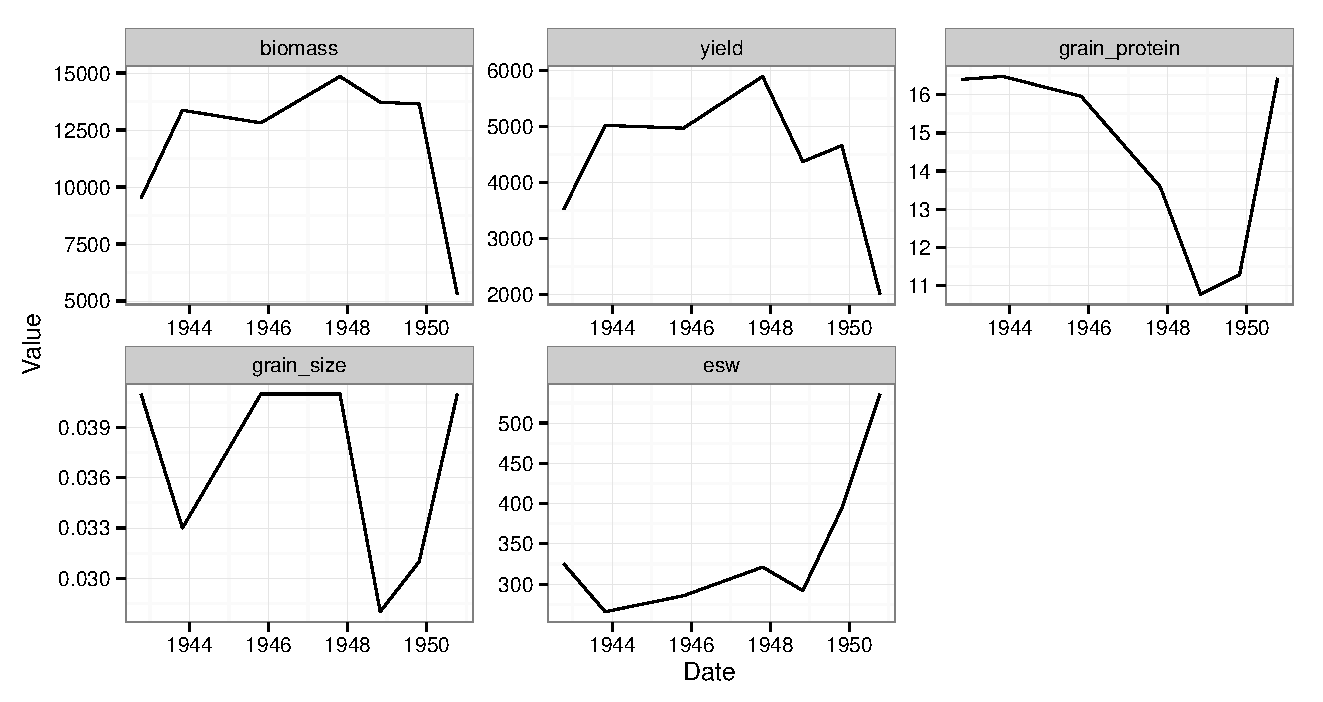
\includegraphics[width=1\textwidth]{figures/allon1.png}
\caption{Figures produced by \code{plot.apsim} with argument \code{one\_plot = TRUE}.}
\label{fig:allon1}
\end{figure}

Plot just yield as a function of time.  See Figure \ref{fig:yield}.
\begin{knitrout}
\definecolor{shadecolor}{rgb}{0.969, 0.969, 0.969}\color{fgcolor}\begin{kframe}
\begin{alltt}
\hlkwd{plot}\hlstd{(results[[}\hlnum{2}\hlstd{]],} \hlkwc{y} \hlstd{=} \hlstr{'yield'}\hlstd{)} \hlopt{+} \hlkwd{geom_line}\hlstd{(}\hlkwc{colour} \hlstd{=} \hlstr{'red'}\hlstd{)} \hlopt{+} \hlkwd{theme_bw}\hlstd{()}
\end{alltt}
\end{kframe}
\end{knitrout}

\begin{figure}[H]
\centering
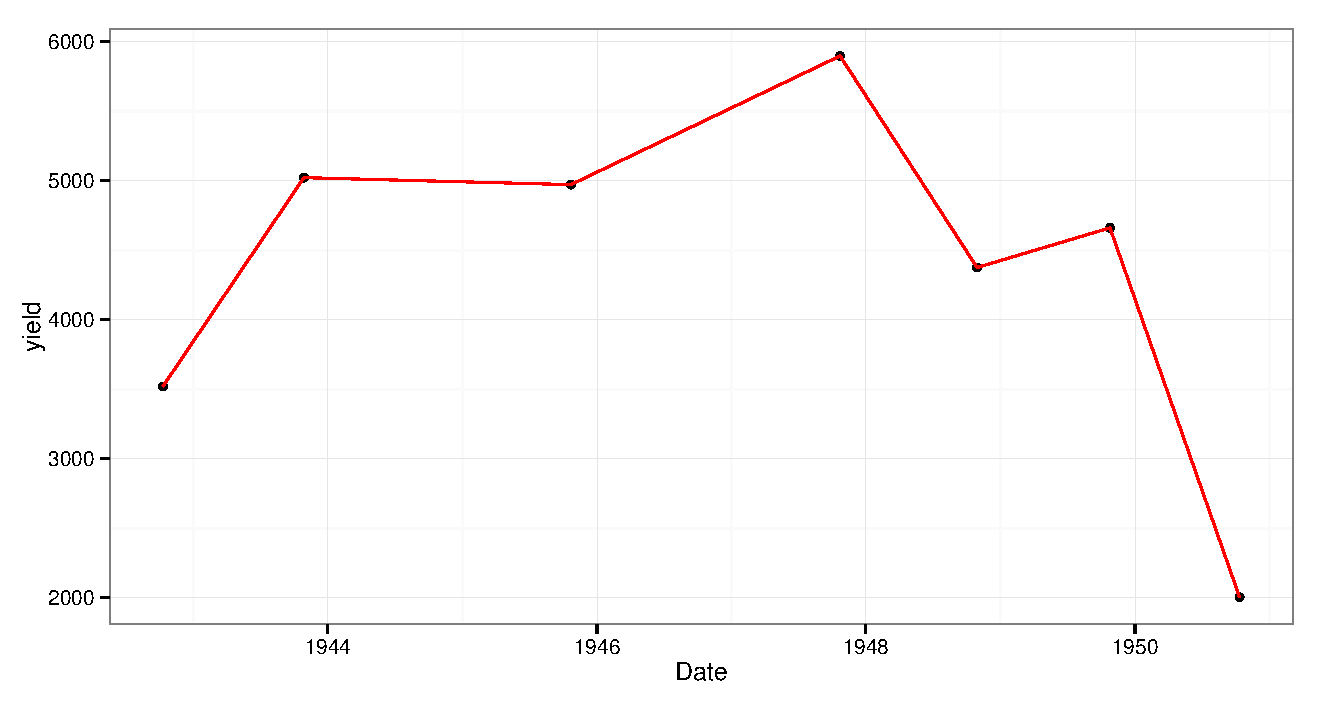
\includegraphics[width=1\textwidth]{figures/yield.png}
\caption{Plot produced by \code{plot.apsim} with argument \code{y = 'yield'}.}
\label{fig:yield}
\end{figure}

\end{document}
